% !TeX program = xelatex
\documentclass[aspectratio=169,11pt]{beamer}

\usepackage{amsmath,booktabs,tikz,colortbl,array}
\usetikzlibrary{positioning}

\definecolor{talknavy}{HTML}{1B3A5C}
\definecolor{talkorange}{HTML}{E07A2F}
\definecolor{talkgreen}{HTML}{2F7A4A}
\definecolor{talkink}{HTML}{1B3A5C}
\definecolor{talkmuted}{HTML}{6B7280}
\definecolor{talkline}{HTML}{D7DEE6}
\definecolor{talkcard}{HTML}{F3F5F8}
\definecolor{talkclean}{HTML}{9AA6B2}
\definecolor{talkbg}{HTML}{FFFFFF}

\setbeamercolor{normal text}{fg=talkink,bg=white}
\setbeamercolor{frametitle}{fg=talknavy,bg=white}
\setbeamercolor{framesubtitle}{fg=talknavy,bg=white}
\setbeamercolor{footline}{fg=talkmuted,bg=white}
\setbeamerfont{frametitle}{size=\Large,series=\bfseries}
\setbeamerfont{framesubtitle}{size=\small}
\setbeamersize{text margin left=8mm,text margin right=8mm}
\setbeamertemplate{navigation symbols}{}

\setbeamertemplate{frametitle}{%
  \vspace{1.6mm}%
  {\usebeamerfont{frametitle}\color{talknavy}\insertframetitle\par}%
  \ifx\insertframesubtitle\@empty\else
    \vspace{0.4mm}{\usebeamerfont{framesubtitle}\color{talknavy}\insertframesubtitle}\fi
  \vspace{2.2mm}%
  {\color{talkline}\hrule height 0.45pt}%
  \vspace{3.2mm}%
}

\setbeamertemplate{footline}{%
  \leavevmode
  \hbox{%
    \begin{beamercolorbox}[wd=.72\paperwidth,ht=2.6ex,dp=1.5ex,leftskip=8mm]{footline}%
      {\scriptsize CISC 7402 \,|\, Routing Robustness in MoE}
    \end{beamercolorbox}%
    \begin{beamercolorbox}[wd=.28\paperwidth,ht=2.6ex,dp=1.5ex,rightskip=8mm]{footline}%
      \hfill{\scriptsize\insertframenumber\,/\,\inserttotalframenumber}
    \end{beamercolorbox}%
  }%
}

\newcommand{\ratebar}[2]{%
  \begin{tikzpicture}[baseline=-0.55ex]
    \fill[#2] (0,0) rectangle ({#1*1.55cm/4.2},0.26cm);
    \node[anchor=west,inner sep=2pt,font=\scriptsize,text=talkink] at ({#1*1.55cm/4.2},0.13cm) {#1};
  \end{tikzpicture}%
}

\newcommand{\softcard}[3]{%
  \begin{tikzpicture}
        \node[fill=talkcard,rounded corners=3pt,text width=2.95cm,minimum height=3.05cm,
          align=center,inner sep=5pt] {{\normalsize\bfseries\color{#1}#2}\\[1.8mm]{\footnotesize #3}};
  \end{tikzpicture}%
}

\begin{document}

\begin{frame}[plain]
  \vspace{16mm}
  {\LARGE\bfseries\color{talknavy} Disentangling Routing Robustness\\[1.2mm] in Mixture-of-Experts\par}
  \vspace{3.5mm}
  {\large\color{talkmuted} Isolating expert-input distortion from routing shifts across perturbations\par}
  \vspace{6mm}
  {\color{talkorange}\rule{\textwidth}{1.15pt}}
  \vspace{3.5mm}
  {\large\bfseries Do Anh Dung \ {\color{talkmuted}$\cdot$} \ Xiangli Qianhui \ {\color{talkmuted}$\cdot$} \ Yang Jian\par}
  \vspace{7mm}
  {\color{talkmuted} CISC 7402 \,|\, 15-Minute Research Presentation}
\end{frame}

\begin{frame}{Talk Roadmap: 15 Minutes}
  \vspace{3mm}
  \renewcommand{\arraystretch}{1.55}
  \begin{tabular}{@{}>{\bfseries}p{2.7cm}p{3.6cm}p{7.2cm}@{}}
    \color{talkmuted}{Time} & \color{talkmuted}{Speaker} & \color{talkmuted}{Core Question} \\
    \midrule
    \rowcolor{talkcard}
    \color{talknavy}{0:00--5:00} & Do Anh Dung & Is rerouting actually to blame? \\
    \rowcolor{white}
    \color{talkorange}{5:00--10:00} & Xiangli Qianhui & Input damage, routing shift, or both? \\
    \rowcolor{talkcard}
    \color{talkgreen}{10:00--15:00} & Yang Jian & Does a steadier router lower error? \\
  \end{tabular}
\end{frame}

\begin{frame}{Route Switching Is a Symptom, Not a Verdict}
  \framesubtitle{Do Anh Dung}
  \vspace{2mm}
  \begin{columns}[c]
    \begin{column}{0.48\textwidth}
      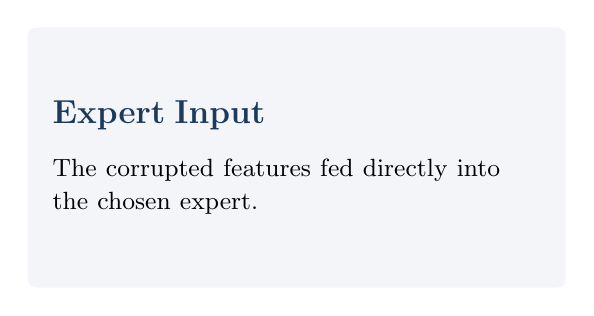
\begin{tikzpicture}
        \node[fill=talkcard,rounded corners=3pt,text width=6.2cm,minimum height=3.3cm,align=left,inner sep=9pt]
          {{\large\bfseries\color{talknavy} Expert Input}\\[2.4mm]
           {\small The corrupted features fed directly into the chosen expert.}};
      \end{tikzpicture}
    \end{column}
    \begin{column}{0.48\textwidth}
      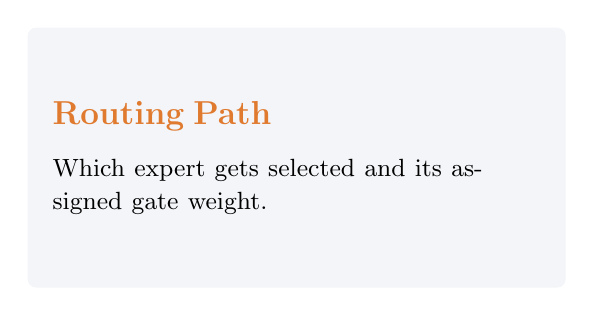
\begin{tikzpicture}
        \node[fill=talkcard,rounded corners=3pt,text width=6.2cm,minimum height=3.3cm,align=left,inner sep=9pt]
          {{\large\bfseries\color{talkorange} Routing Path}\\[2.4mm]
           {\small Which expert gets selected and its assigned gate weight.}};
      \end{tikzpicture}
    \end{column}
  \end{columns}
  \vspace{7mm}
  {\large\textbf{Takeaway:} Switch rate counts flips; it never prices their impact on accuracy.}
\end{frame}

\begin{frame}{One Trained Model, Four Paired Evaluations}
  \framesubtitle{Do Anh Dung}
  \vspace{-1mm}
  \centering
  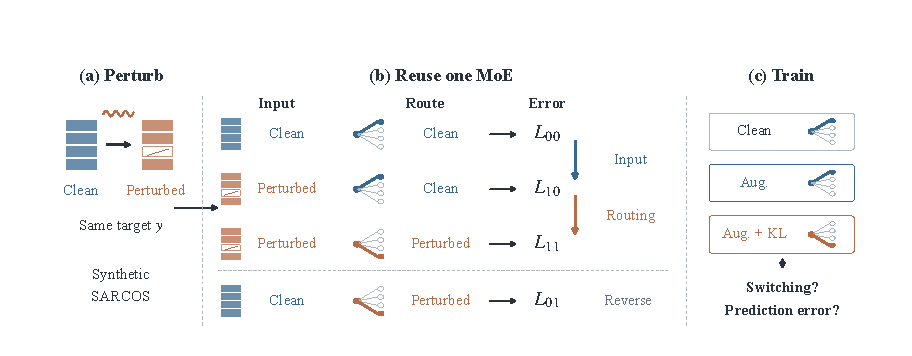
\includegraphics[width=\linewidth,height=0.72\textheight,keepaspectratio]{figures/four_cells.pdf}
\end{frame}

\begin{frame}{Fixed Input $u$, Four Distinct Maps}
  \framesubtitle{Do Anh Dung \hspace{2mm}$\cdot$\hspace{2mm} Task cue $e_c$ governs the target function}
  \vspace{1mm}
  \centering
  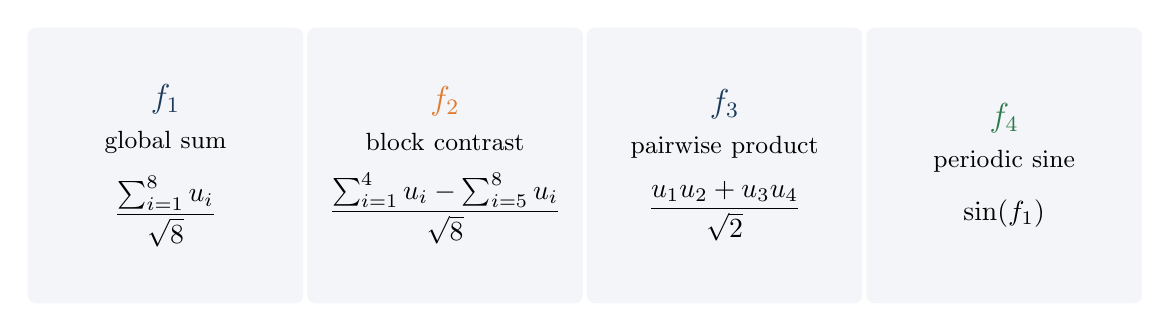
\begin{tikzpicture}
    \node[fill=talkcard,rounded corners=3pt,text width=3.15cm,minimum height=3.5cm,align=center,inner sep=5pt]
      at (0,0) {{\large\bfseries\color{talknavy}$f_1$}\\[1mm]{\small global sum}\\[2.5mm]
      $\displaystyle\frac{\sum_{i=1}^{8}u_i}{\sqrt{8}}$};
    \node[fill=talkcard,rounded corners=3pt,text width=3.15cm,minimum height=3.5cm,align=center,inner sep=5pt]
      at (3.55,0) {{\large\bfseries\color{talkorange}$f_2$}\\[1mm]{\small block contrast}\\[2.5mm]
      $\displaystyle\frac{\sum_{i=1}^{4}u_i-\sum_{i=5}^{8}u_i}{\sqrt{8}}$};
    \node[fill=talkcard,rounded corners=3pt,text width=3.15cm,minimum height=3.5cm,align=center,inner sep=5pt]
      at (7.1,0) {{\large\bfseries\color{talknavy}$f_3$}\\[1mm]{\small pairwise product}\\[2.5mm]
      $\displaystyle\frac{u_1u_2+u_3u_4}{\sqrt{2}}$};
    \node[fill=talkcard,rounded corners=3pt,text width=3.15cm,minimum height=3.5cm,align=center,inner sep=5pt]
      at (10.65,0) {{\large\bfseries\color{talkgreen}$f_4$}\\[1mm]{\small periodic sine}\\[2.5mm]
      $\sin(f_1)$};
  \end{tikzpicture}

  \vspace{7mm}
  {\small\textbf{\color{talknavy}$u$: predictive} \hspace{3mm}{\color{talkmuted}$\cdot$} \hspace{3mm} $v$: nuisance
  \hspace{3mm}{\color{talkmuted}$\cdot$} \hspace{3mm} {\color{talkorange} shortcut injects $2e_c$ during training only}}
\end{frame}

\begin{frame}{Experts Clearly Specialize}
  \framesubtitle{Xiangli Qianhui \hspace{2mm}$\cdot$\hspace{2mm} Independent training profile}
  \vspace{-1.5mm}
  \centering
  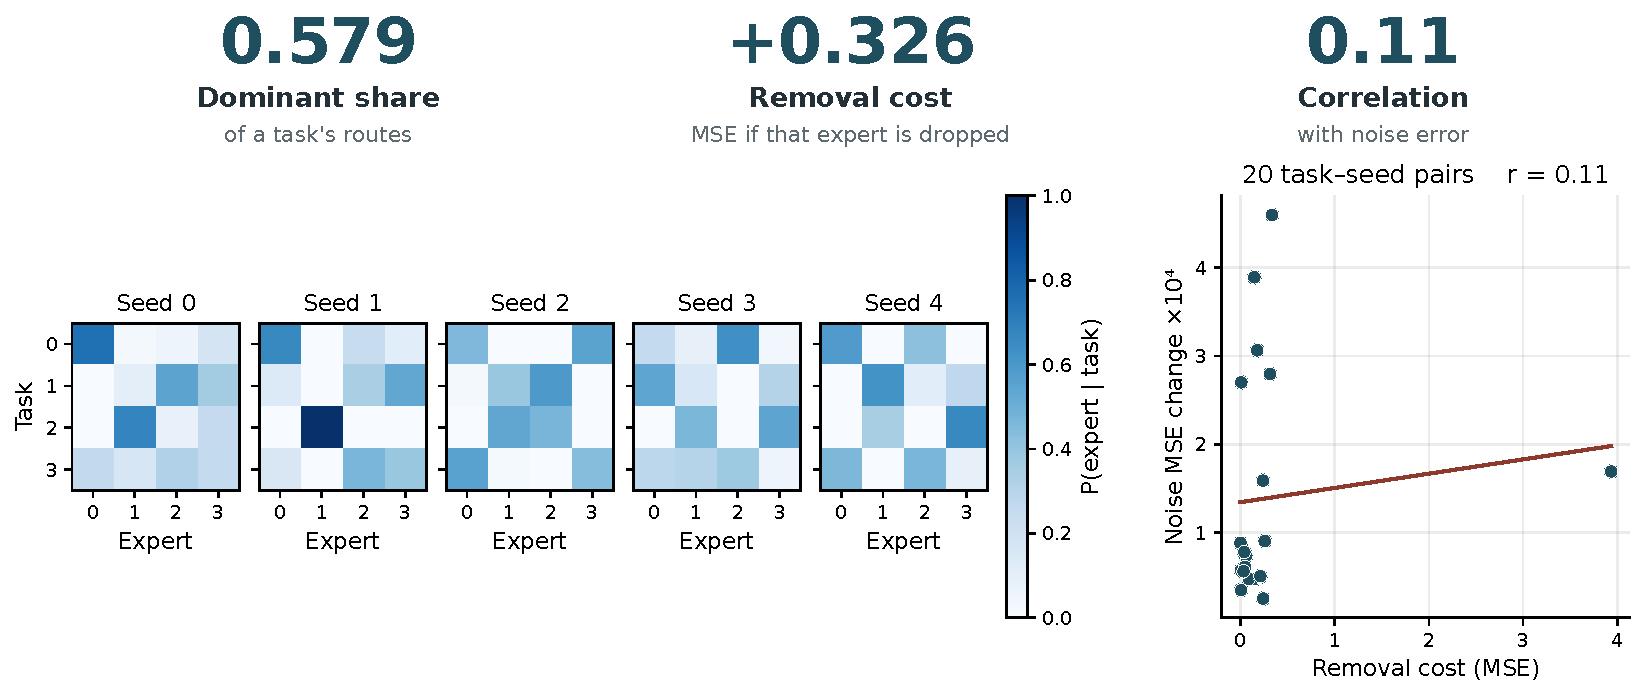
\includegraphics[width=\linewidth,height=0.74\textheight,keepaspectratio]{figures/specialization.pdf}
\end{frame}

\begin{frame}{Task Preserved: Rerouting Plays Multiple Roles}
  \framesubtitle{Xiangli Qianhui \hspace{2mm}$\cdot$\hspace{2mm} $\Delta$MSE $\times 10^{4}$ with 95\% bootstrap intervals}
  \vspace{-1.5mm}
  \centering
  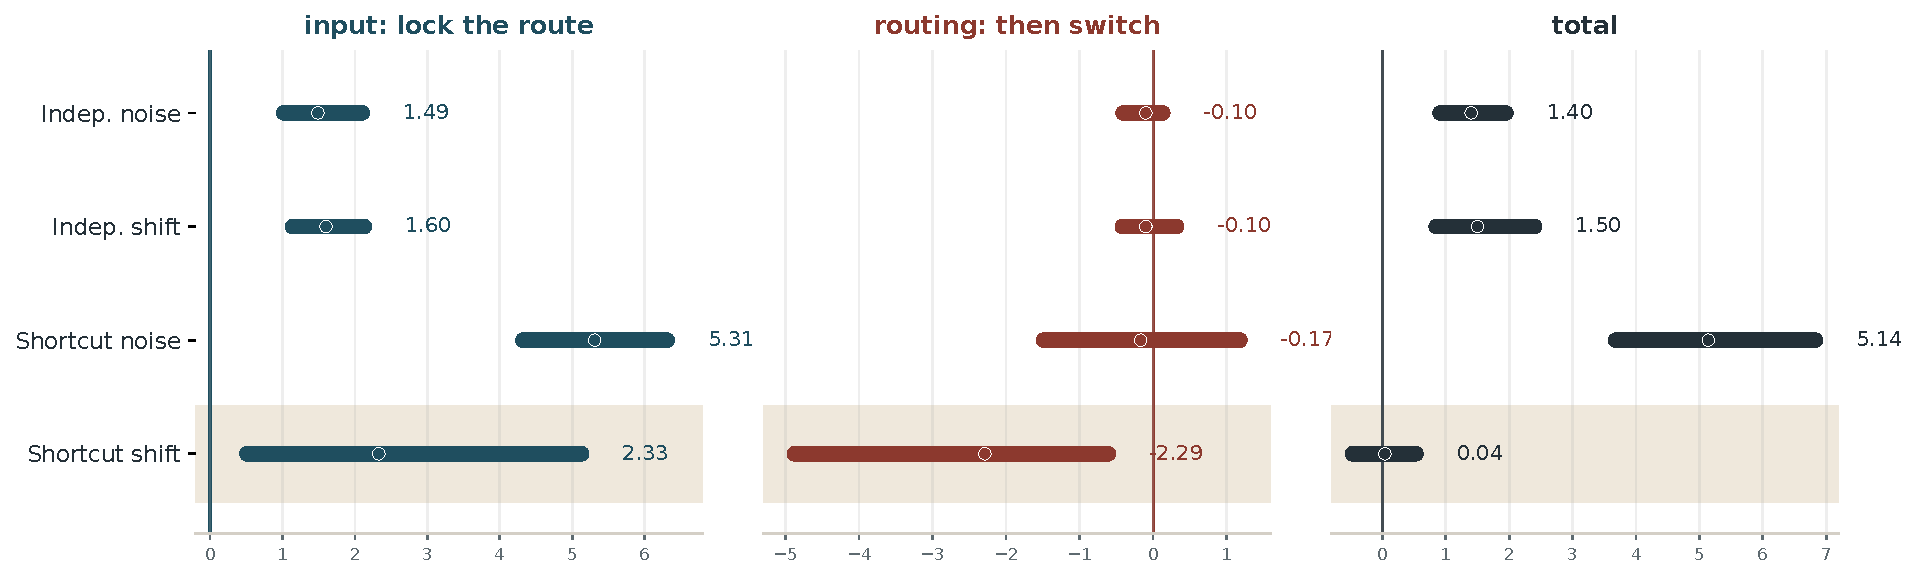
\includegraphics[width=\linewidth,height=0.62\textheight,keepaspectratio]{figures/task_kept.pdf}\\[1mm]
  {\small The first three red bars sit near zero. Under shortcut shift, routing turns negative and cancels input damage.}
\end{frame}

\begin{frame}{Information Loss Splits Into Two Regimes}
  \framesubtitle{Xiangli Qianhui \hspace{2mm}$\cdot$\hspace{2mm} Independent profile, raw MSE}
  \vspace{-1.5mm}
  \centering
  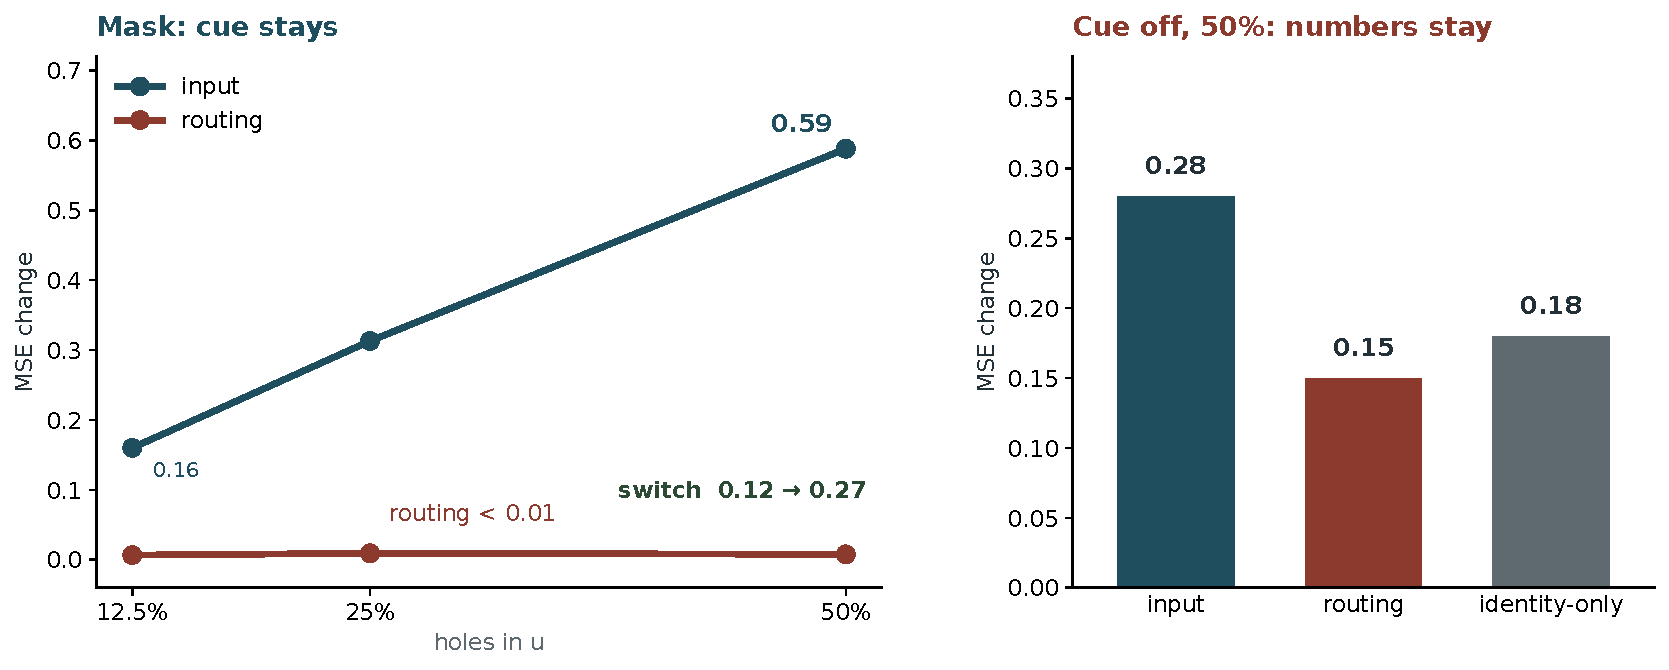
\includegraphics[width=\linewidth,height=0.62\textheight,keepaspectratio]{figures/delete_info.pdf}\\[1mm]
  {\small Feature masking: routing stays flat as switching climbs. Cue removal: both terms add error.}
\end{frame}

\begin{frame}{Dense Baselines: Advantage Hinges on the Perturbation}
  \framesubtitle{Xiangli Qianhui \hspace{2mm}$\cdot$\hspace{2mm} Independent profile}
  \vspace{-1.5mm}
  \centering
  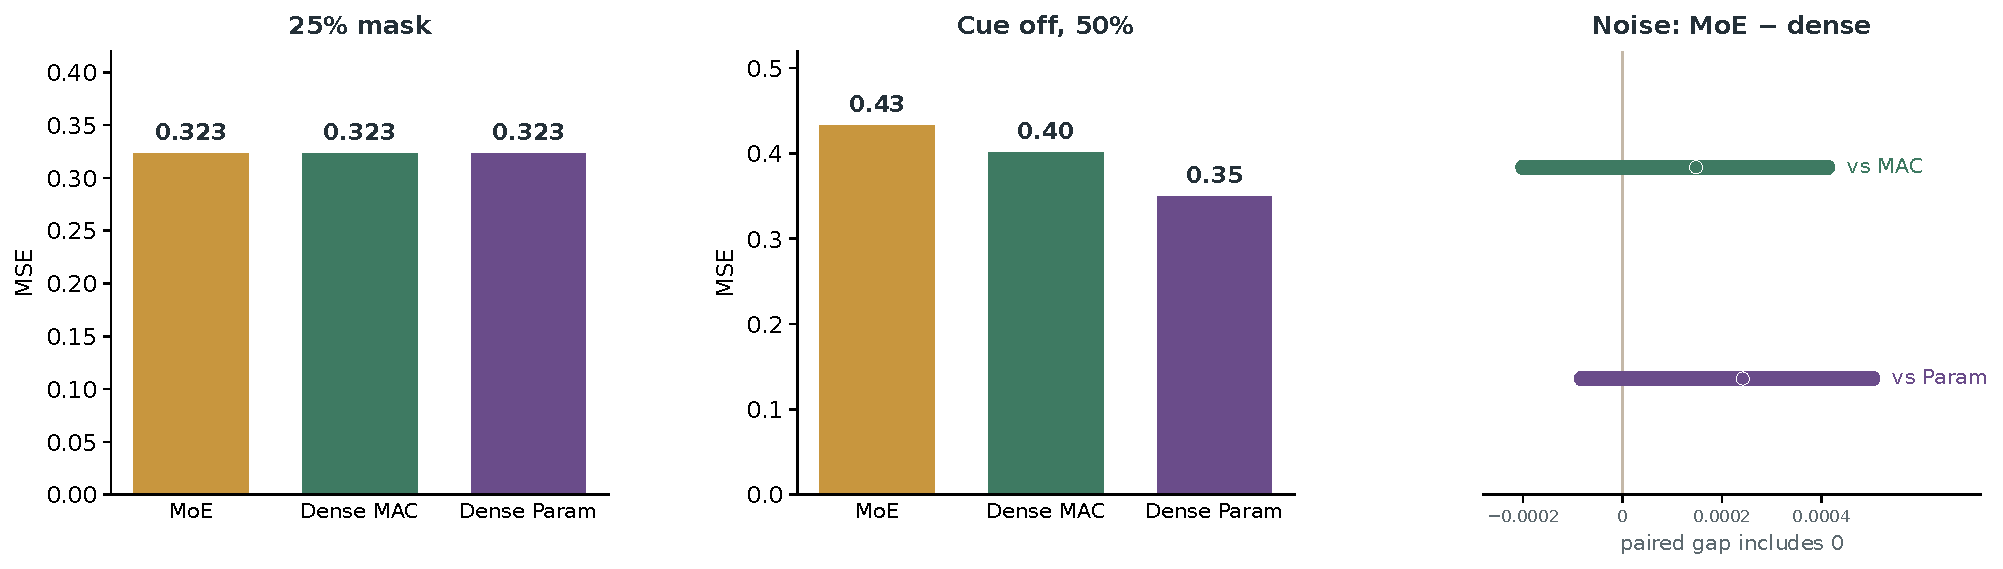
\includegraphics[width=\linewidth,height=0.62\textheight,keepaspectratio]{figures/dense_gap.pdf}\\[1mm]
  {\small Matched under feature masking; MoE lags once the cue disappears; noise gaps span zero.}
\end{frame}

\begin{frame}{A Lower Mean Curve Is Not a Confirmed Gain}
  \framesubtitle{Yang Jian \hspace{2mm}$\cdot$\hspace{2mm} Synthetic nuisance noise}
  \vspace{-1.5mm}
  \centering
  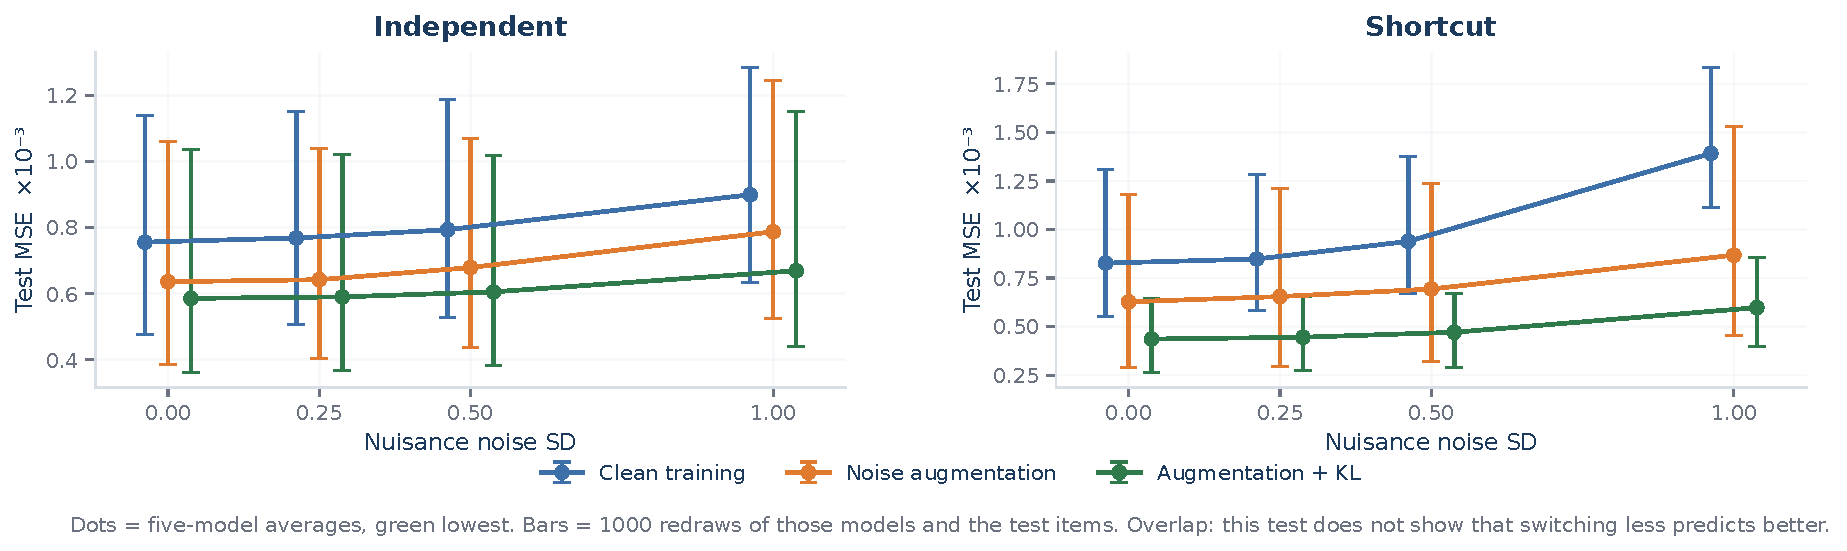
\includegraphics[width=\linewidth,height=0.62\textheight,keepaspectratio]{figures/train_curves.pdf}\\[1mm]
  {\small Dots: five-model averages, green lowest. Bars: 1000 redraws of those models and the test items. Overlap: this test does not show that switching less predicts better.}
\end{frame}

\begin{frame}{Where Routing Stability Actually Improves}
  \framesubtitle{Yang Jian \hspace{2mm}$\cdot$\hspace{2mm} Expert switch rate $\times 100$}
  {\small\color{talkclean}\rule{4mm}{1.5mm}}\ clean \hspace{4mm}
  {\small\color{talkorange}\rule{4mm}{1.5mm}}\ augmentation \hspace{4mm}
  {\small\color{talkgreen}\rule{4mm}{1.5mm}}\ consistency\\[2.8mm]
  \renewcommand{\arraystretch}{1.45}
  \begin{tabular}{@{}lccc@{}}
    \color{talkmuted}{\textbf{Condition}} & \color{talkmuted}{\textbf{Clean}} & \color{talkmuted}{\textbf{Augmentation}} & \color{talkmuted}{\textbf{Consistency}} \\
    \midrule
    \rowcolor{talkcard}
    Indep.\ noise & \ratebar{2.88}{talkclean} & \ratebar{2.30}{talkorange} & \ratebar{1.60}{talkgreen} \\
    Indep.\ shift & \ratebar{3.18}{talkclean} & \ratebar{3.11}{talkorange} & \ratebar{1.53}{talkgreen} \\
    \rowcolor{talkcard}
    Shortcut noise & \ratebar{4.00}{talkclean} & \ratebar{3.15}{talkorange} & \ratebar{1.09}{talkgreen} \\
    Shortcut shift & \ratebar{4.09}{talkclean} & \ratebar{2.56}{talkorange} & \ratebar{0.99}{talkgreen} \\
  \end{tabular}\\[3.5mm]
  {\small Augmentation already captures much of the stability gain; consistency cuts switches further without proven accuracy gains.}
\end{frame}

\begin{frame}{SARCOS: Same Pattern, One Helpful Exception}
  \framesubtitle{Yang Jian}
  \vspace{-1.5mm}
  \centering
  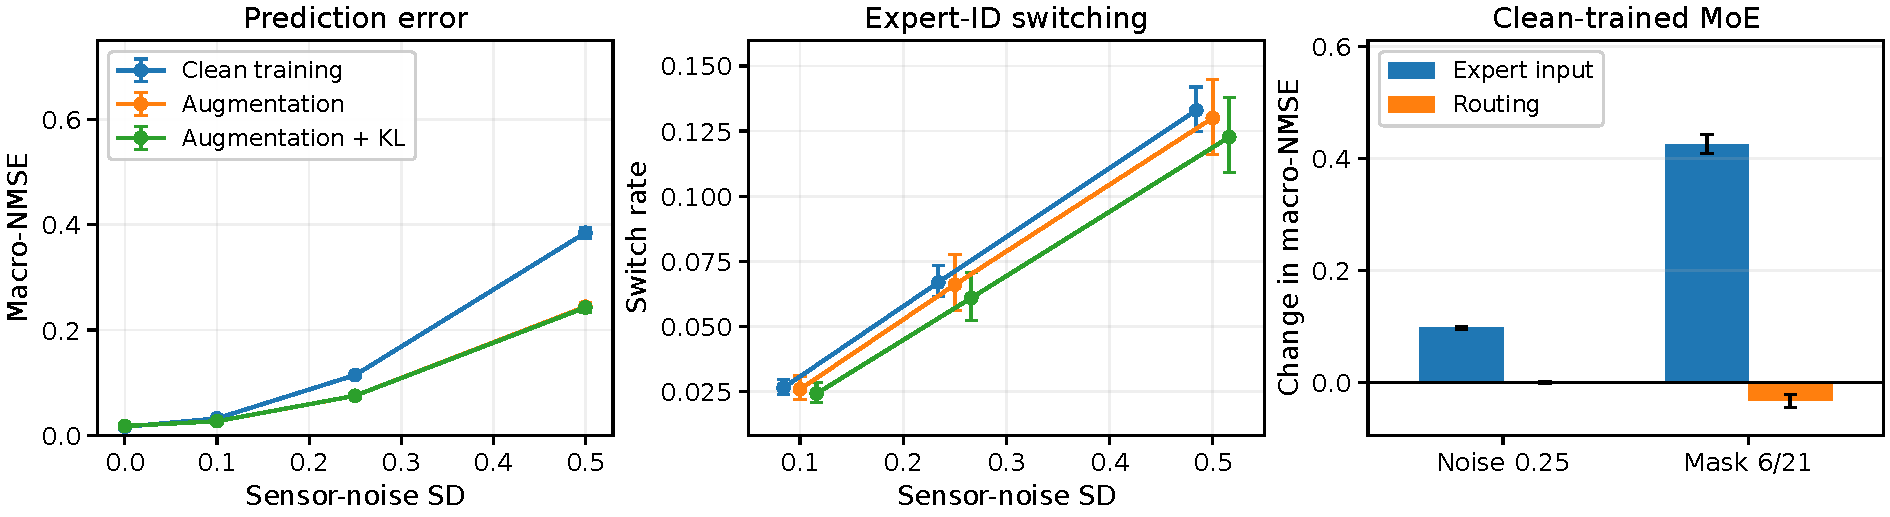
\includegraphics[width=\linewidth,height=0.60\textheight,keepaspectratio]{figures/sarcos.pdf}\\[1.2mm]
  \raggedright
  {\small Key exception: when masking 6 of 21 sensors, routing contributes $-0.032$ [$-0.044$, $-0.020$], actively cushioning input loss.}
\end{frame}

\begin{frame}{Three Takeaways From Fifteen Minutes}
  \framesubtitle{Yang Jian}
  \vspace{2mm}
  \renewcommand{\arraystretch}{1.7}
  \begin{tabular}{@{}>{\bfseries}p{1.1cm}p{12.6cm}@{}}
    \color{talkmuted}{\#} & \color{talkmuted}{Key Finding} \\
    \midrule
    \rowcolor{talkcard}
    \color{talknavy}{01} & When noise raises error, experts mainly read dirty inputs. \\
    \rowcolor{white}
    \color{talkorange}{02} & Switching can do little, offset damage, or add error---depends on the test, not switch count alone. \\
    \rowcolor{talkcard}
    \color{talkgreen}{03} & Training for fewer switches does not establish more accurate predictions. \\
  \end{tabular}
\end{frame}

\begin{frame}{Boundaries of Our Scope}
  \framesubtitle{Yang Jian}
  \vspace{1.5mm}
  \centering
  \softcard{talkorange}{Top-1 MLPs}{Four small MLP experts rather than large language models.}
  \hspace{3mm}
  \softcard{talkorange}{Path order}{Input-first and route-first attributions can diverge.}
  \hspace{3mm}
  \softcard{talkgreen}{Single arm}{Real-data validation covers one SARCOS robotics archive.}
\end{frame}

\begin{frame}[plain]
  \vspace{22mm}
  \centering
  {\LARGE\bfseries\color{talknavy} Thank you for watching.\par}
  \vspace{8mm}
  {\color{talkorange}\rule{16mm}{1.2pt}}
  \hspace{2mm}
  {\large Do Anh Dung \ {\color{talkmuted}$\cdot$} \ Xiangli Qianhui \ {\color{talkmuted}$\cdot$} \ Yang Jian}
\end{frame}

\end{document}
